\section{Observation and Calculations}

\subsection{Energy calibration of scintillation detector}
At first, the scintillation detector is calibrated using a mixed source of Americum and Cesium. The resulting spectra is shown in Fig. \ref{calib}. The two peaks are calibrated to 59.54 keV (due to Am-241) and 661.66 keV (due to Cs-137). 

\begin{figure}[H]
    \centering
    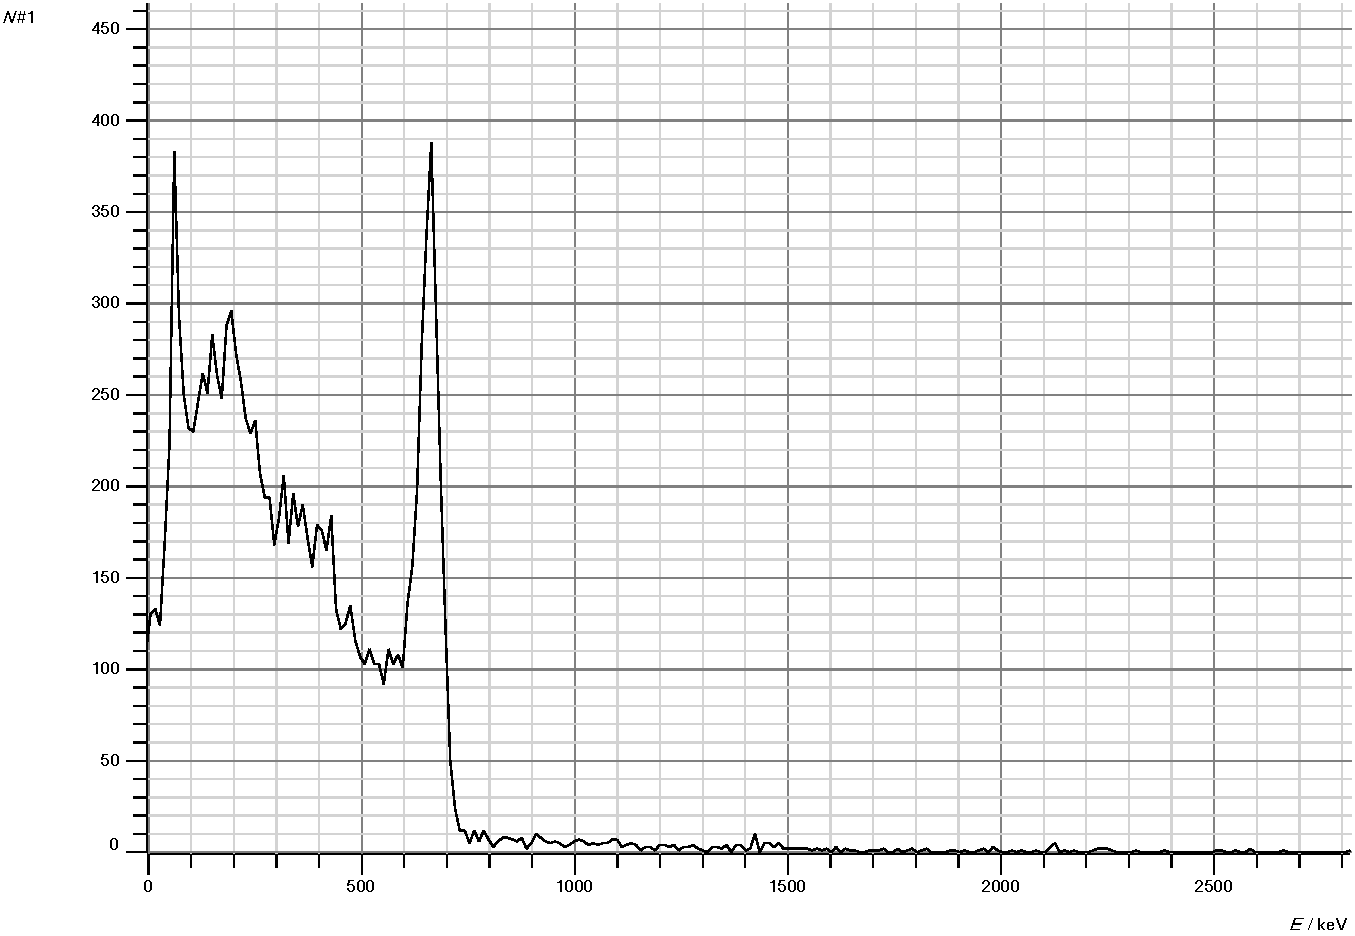
\includegraphics[width=1\columnwidth]{images/al_calib.pdf}
    \caption{Energy Callibration Curve}
    \label{calib}
\end{figure}

\subsection{Change in wavelength of the scattered $\gamma$ radiation as a function the $\theta$}

The scattering spectra observed for different scattering angles are shown in Fig. \ref{plot1}. A gaussian is fitted for each peak and the best-fit $\mu$ value corresponds to $E_\theta$. Tables I and II summarise the corresponding $\Delta E$ and $\Delta \lambda$ values for both the scattering bodies.

\begin{figure*}
    \begin{subfigure}{\linewidth}
        \centering
        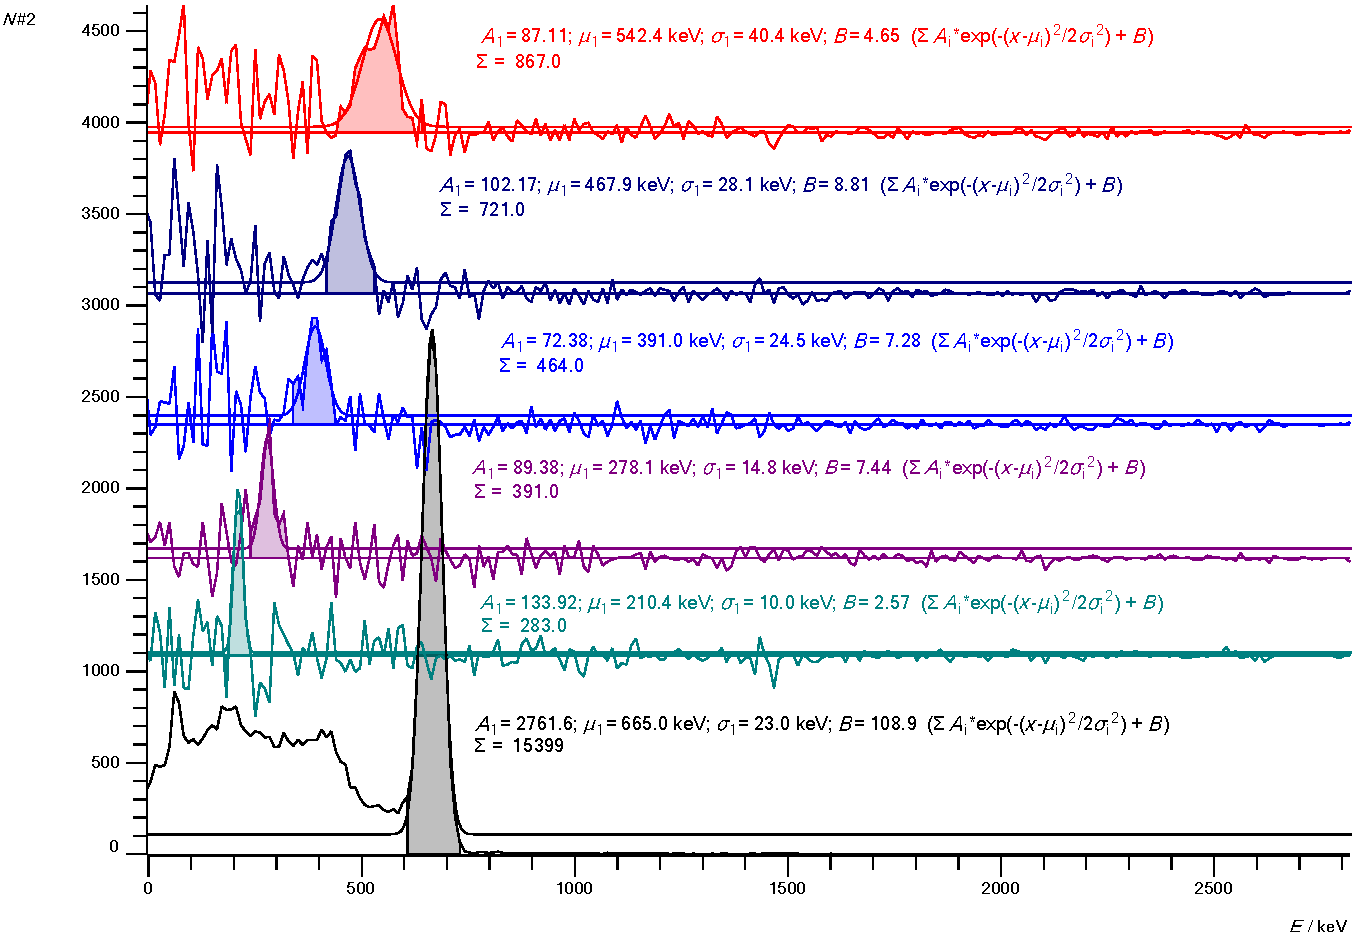
\includegraphics[width=0.9\columnwidth]{images/al_counts.pdf}
        \caption{Aluminium scattering body}
    \end{subfigure}
    \begin{subfigure}{\linewidth}
        \centering
        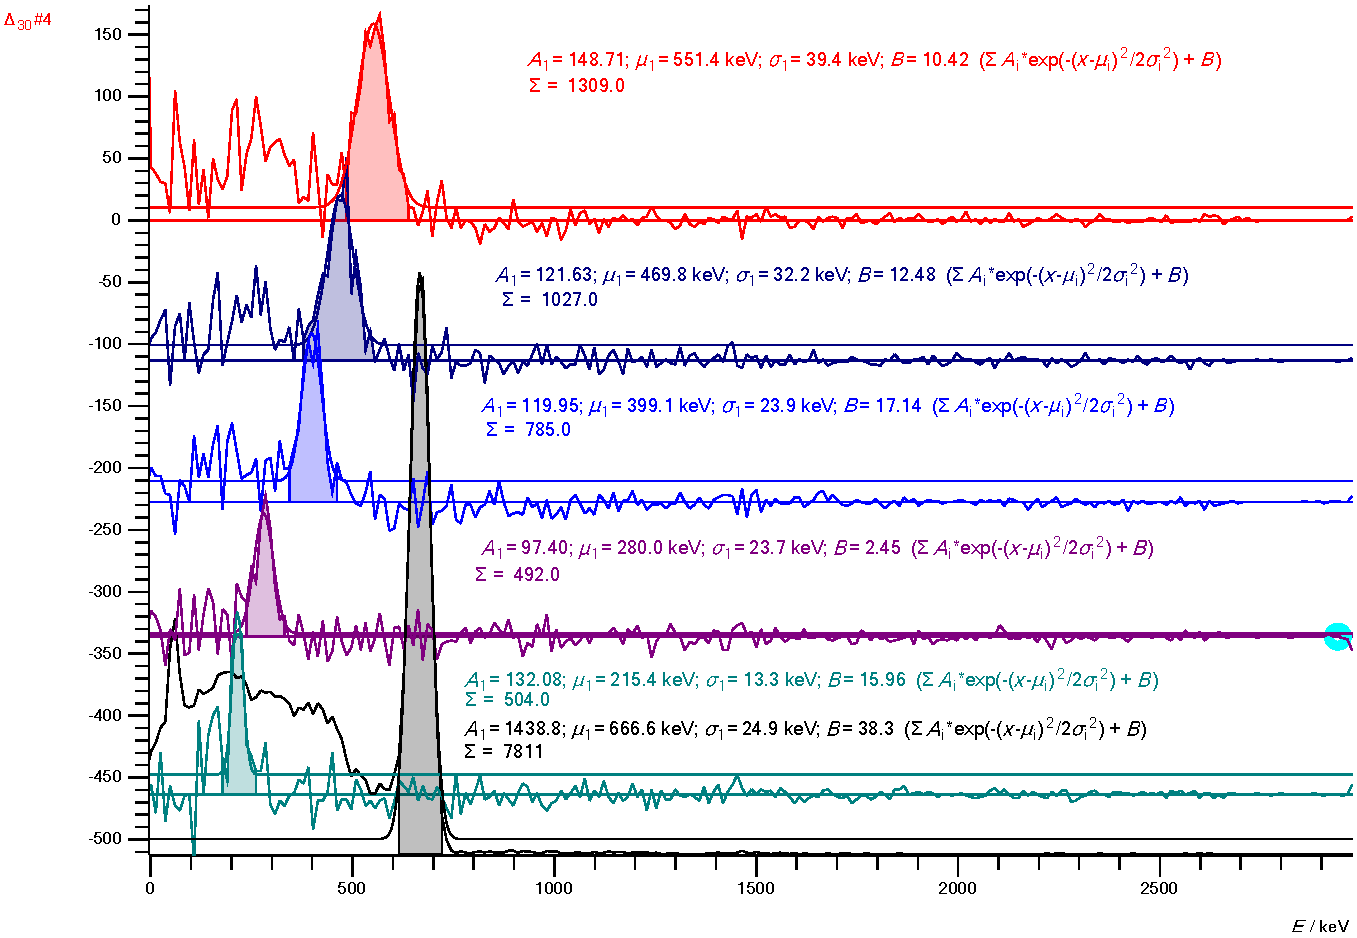
\includegraphics[width=0.9\columnwidth]{images/cu_counts.pdf}
        \caption{Copper scattering body}
    \end{subfigure}
    \caption{Scattering Spectra due to Compton scattering for different scattering angles}
    \label{plot1}
\end{figure*}

\begin{table}[H]
    \centering
    \begin{tabular}{|c|c|c|c|c|c|c|}
    \hline
    $\theta$ & $E$ & $\Delta E_\text{obs}$ & $\Delta E_\text{th}$ & $\lambda$ & $\Delta \lambda_\text{obs}$ & $\Delta \lambda_\text{th}$ \\
    ($^\circ$) & (keV) & (keV) & (keV) & (pm) & (pm) & (pm) \\ \hline
    0 & 665.0 & 0.0 & 0.0 & 1.86 & 0 & 0.000 \\ \hline
    30 & 542.4 & 122.6 & 97.9 & 2.29 & 0.421 & 0.325 \\ \hline
    45 & 467.9 & 197.1 & 182.1 & 2.65 & 0.785 & 0.711 \\ \hline
    60 & 391.0 & 274.0 & 260.2 & 3.17 & 1.307 & 1.213 \\ \hline
    90 & 278.1 & 386.9 & 373.6 & 4.46 & 2.594 & 2.426 \\ \hline
    120 & 210.4 & 454.6 & 437.1 & 5.89 & 4.029 & 3.639 \\ \hline
    \end{tabular}
    \caption{$E$ and the corresponding $\Delta E$ and $\Delta \lambda$ values as function of $\theta$ for the Aluminium scattering body based on Fig. \ref{plot1}.}
    \label{tab:1}
\end{table}
\begin{table}[H]
    \centering
    \begin{tabular}{|c|c|c|c|c|c|c|}
    \hline
    $\theta$ & $E$ & $\Delta E_\text{obs}$ & $\Delta E_\text{th}$ & $\lambda$ & $\Delta \lambda_\text{obs}$ & $\Delta \lambda_\text{th}$ \\
    ($^\circ$) & (keV) & (keV) & (keV) & (pm) & (pm) & (pm) \\ \hline
    0 & 666.6 & 0.0 & 0.0 & 1.86 & 0 & 0.000 \\ \hline
    30 & 551.4 & 115.2 & 97.9 & 2.25 & 0.389 & 0.325 \\ \hline
    45 & 469.8 & 196.8 & 182.1 & 2.64 & 0.779 & 0.711 \\ \hline
    60 & 399.1 & 267.5 & 260.2 & 3.11 & 1.247 & 1.213 \\ \hline
    90 & 280.0 & 386.6 & 373.6 & 4.43 & 2.568 & 2.426 \\ \hline
    120 & 215.4 & 451.2 & 437.1 & 5.76 & 3.897 & 3.639 \\ \hline
    \end{tabular}
    \caption{$E$ and the corresponding $\Delta E$ and $\Delta \lambda$ values as function of $\theta$ for the Copper scattering body based on Fig. \ref{plot1}.}
    \label{tab:2}
\end{table}

Fig. \ref{plot3} shows the variation in experimental and theoretical $\Delta \lambda$ values as a function of $\theta$.

\begin{figure}[H]
    \begin{subfigure}{\linewidth}
        \centering
        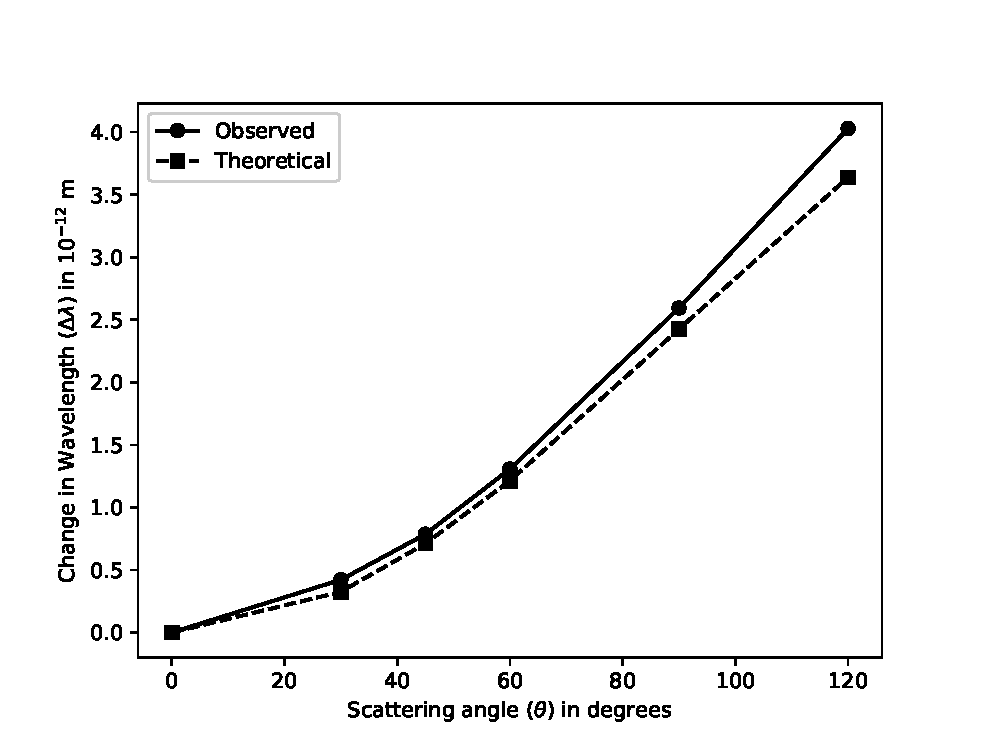
\includegraphics[width=1\columnwidth]{images/al.eps}
        \caption{Aluminium scattering body}
    \end{subfigure}
\end{figure}
\begin{figure}[H]
    \ContinuedFloat
    \begin{subfigure}{\linewidth}
        \centering
        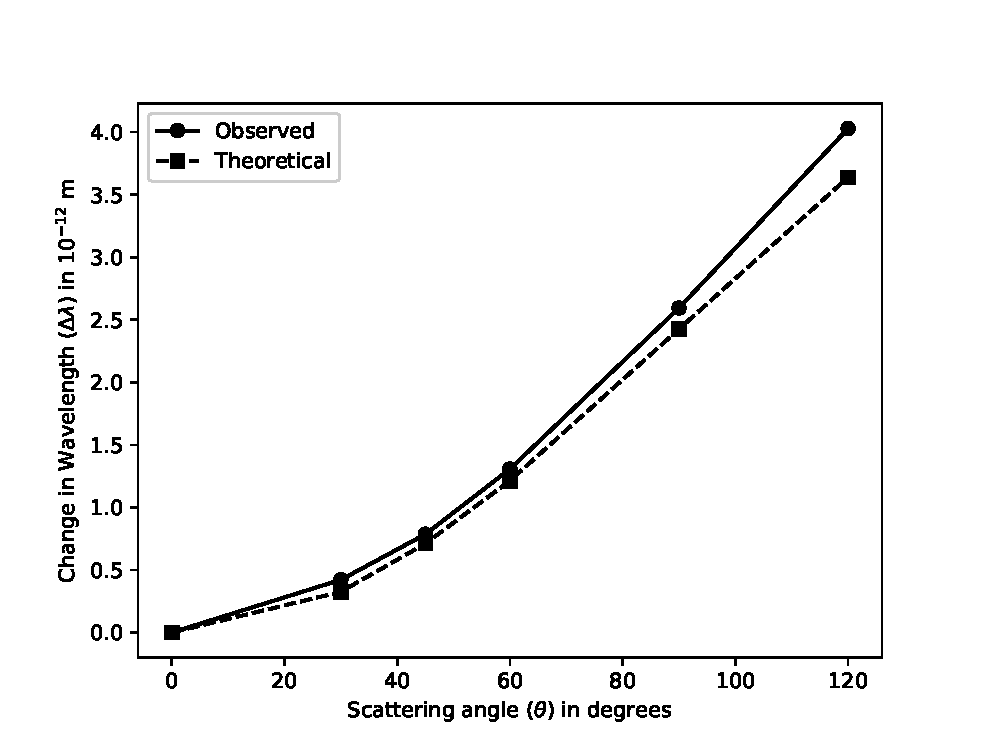
\includegraphics[width=1\columnwidth]{images/al.eps}
        \caption{Copper scattering body}
    \end{subfigure}
    \caption{Comparison of Wavelength shift due to Compton scattering for copper theoretically and experimentally}
    \label{plot3}
\end{figure}

\vspace{2em}

Fig. \ref{plot2} shows the variation in $E$ as a function of $\theta$. The data points have been fitted to the function based on Eq. 4,

\begin{align*}
    E = \frac{662}{1+\frac{662}{511}(1-\cos \theta)}
\end{align*}

where $E_0$ is 662 keV and $m_ec^2$ is 511 keV. We can see that our data agrees with the theoretical predictions with a pretty good $r$-value.

\begin{figure}[H]
    \begin{subfigure}{\linewidth}
        \centering
        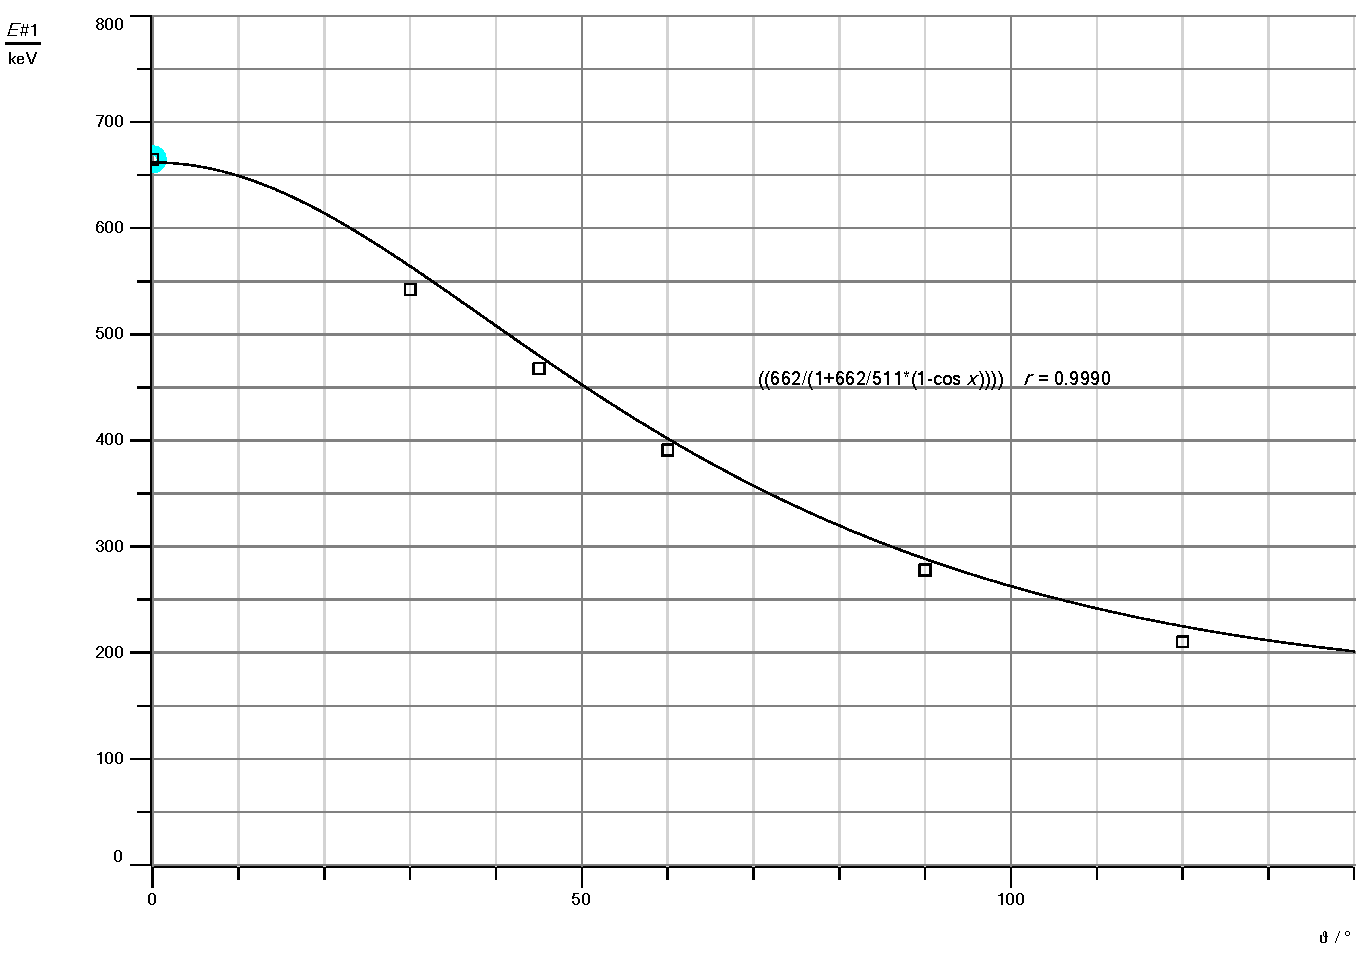
\includegraphics[width=1\columnwidth]{images/al_fit.pdf}
        \caption{Aluminium scattering body, $r$-value = 0.9990}
    \end{subfigure}
\end{figure}
\begin{figure}[H]
    \ContinuedFloat
    \begin{subfigure}{\linewidth}
        \centering
        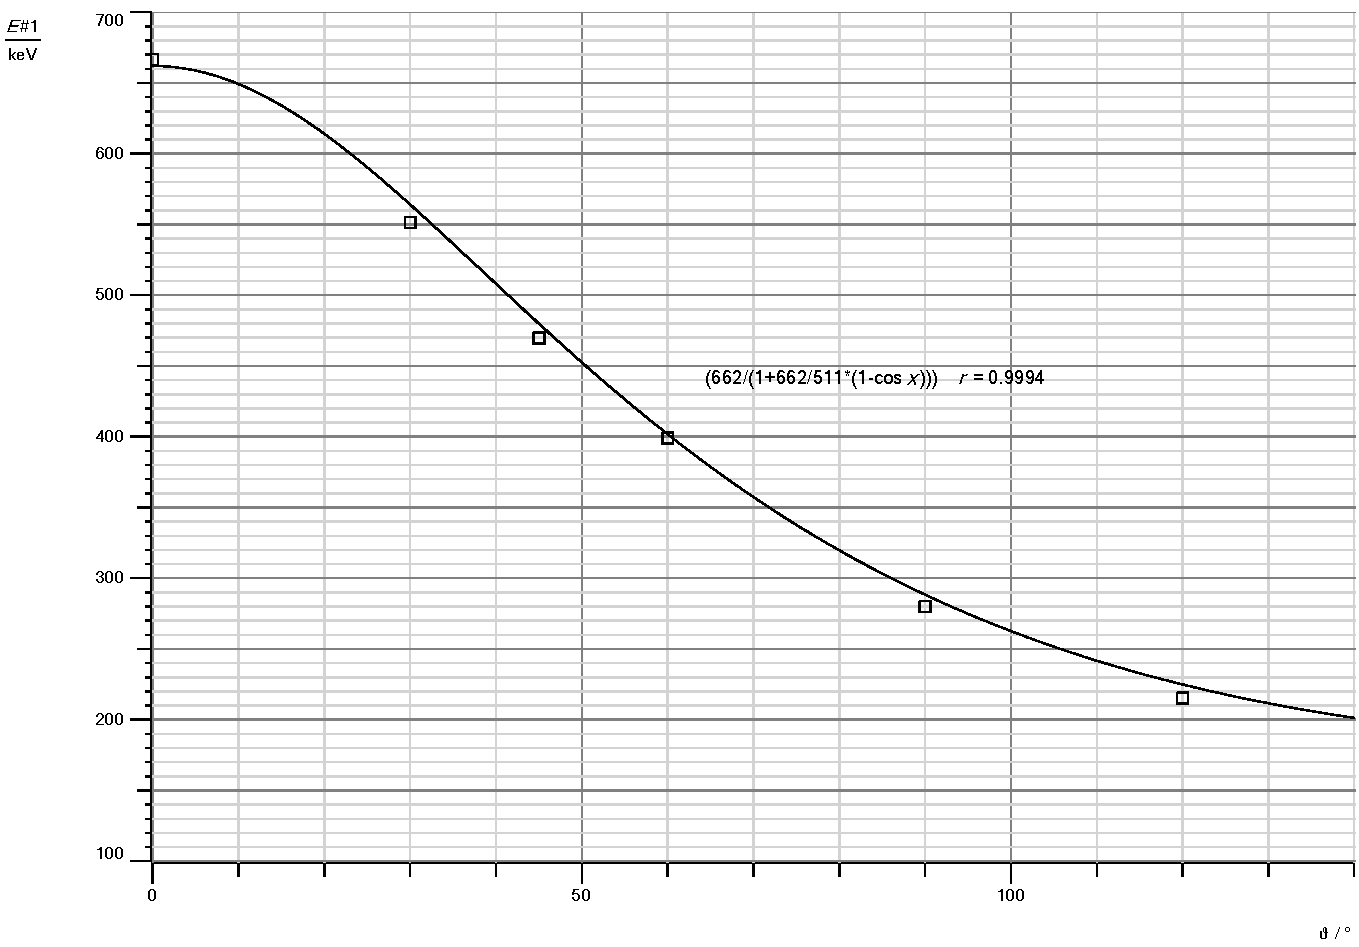
\includegraphics[width=1\columnwidth]{images/cu_fit.pdf}
        \caption{Copper scattering body, $r$-value = 0.9994}
    \end{subfigure}
    \caption{Energy vs Scattering angle due to Compton scattering for different scattering angles}
    \label{plot2}
\end{figure}


\subsection{Calculation of Differential cross-section and the Calibration Factor}

Talble III shows the intensity distribution across different scattering angles measured from the area under the peaks from Fig. \ref{plot1}. The differential cross section has been calculated from Eq. 5.\\

\begin{table}[H]
    \centering
    \begin{tabular}{|c|c|c|c|}
    \hline
    $\theta$ & $\frac{d\sigma}{d\Omega}$ & $I_\theta$ for Al & $I_\theta$ for Cu \\
    ($^\circ$) & ($\times 10^{-30}$ m$^2$) &  &  \\ \hline
    0 & 7.941 & 15399 & 7811 \\ \hline
    30 & 6.890 & 867 & 1309 \\ \hline
    45 & 5.733 & 721 & 1027 \\ \hline
    60 & 4.513 & 464 & 785 \\ \hline
    90 & 2.994 & 391 & 492 \\ \hline
    120 & 2.569 & 283 & 504 \\ \hline
    \end{tabular}
    \caption{Differential cross section and observed intensity distribution across different scattering angles for both the scattering bodies}
    \label{tab:3}
\end{table}

Now, using Eq. 6, the Calibration Factor ($C$) can be calculated. This comes out as,

\begin{itemize}
    \item Al: $2.11\times 10^{31}$ m$^{-2}$
    \item Cu: $1.57 \times 10^{31}$ m$^{-2}$
\end{itemize}

\section{Error Analysis}

The error in the calibration factor can be calculated using

\begin{align}
    \frac{\Delta C}{C} = \sqrt{\sum_{i=0}^n \frac{\Delta \frac{d\sigma}{d\Omega}}{\frac{d\sigma}{d\Omega}}}
\end{align}

Plugging in the values the error comes out ot be $0.017 \times 10^{31}$ m$^{-2}$.